\subsubsection{Esiti verifiche sui documenti}
\label{sub:esiti_verifiche_sui_documenti}
Sui documenti sono state utilizzate le metriche per:
    \begin{itemize}
        \item \textbf{Indice di Gulpease};
        \item \textbf{Correttezza lessicale/ortografica}.
    \end{itemize}
Per evitare risultati errati nel calcole dell'Indice di Gulpease si è deciso di non tenere in considerazione:
    \begin{itemize}
        \item Il frontespizio di ogni documento;
        \item Le tabelle presenti nei documenti;
        \item Il diario delle modifiche all'interno di ogni documento.
    \end{itemize}
Per quanto riguarda la correttezza lessicale/ortografica, gli errori trovati non verranno classificati ma semplicemente conteggiati uniformemente includendo anche errori derivati dal mancato rispetto delle convenzioni scritte nelle \textsc{Norme di Progetto v3.11-2.4.1}.
\\ Per ogni metrica di ogni documento verrà inoltre inserito l'esito dell'analisi che può avere risultato soddisfacente o non.

\paragraph{Norme di Progetto}
\label{sub:norme_di_progetto}
Le \textsc{Norme di Progetto v3.11-2.4.1} ha subito poche modifiche che sono state revisionate in sole 2 fasi di approvazione del documento.
Il suo indice di Gulpease si è assestato sul valore 71.

\rowcolors{2}{white!80!lightgray!90}{white}
\renewcommand{\arraystretch}{2} % allarga le righe con dello spazio sotto e sopra
\begin{longtable}[H]{>{\centering\bfseries}m{6cm} >{\centering}m{2cm} >{\centering}m{2.5cm} >{\centering}m{2.5cm} >{\centering\arraybackslash}m{2.5cm}}  
  \rowcolor{lightgray}
  {\textbf{Documento}} & {\textbf{Risultato indice}} & {\textbf{Errori presenti}} & {\textbf{Esito indice}} & {\textbf{Esito errori}}  \\
  \endfirsthead%
  \rowcolor{lightgray}
  {\textbf{Documento}} & {\textbf{Risultato indice}} & {\textbf{Errori presenti}} & {\textbf{Esito indice}} & {\textbf{Esito errori}}  \\
  \endhead%
  \textbf{Norme di Progetto v3.11-2.4.1} & 71               & 0               & Soddisfatto & Soddisfatto \\
  \caption{Risultati metriche per le Norme di Progetto v3.11-2.4.1}
  \label{tab:my-table}
\end{longtable}

\begin{figure}[H]
  \centering
  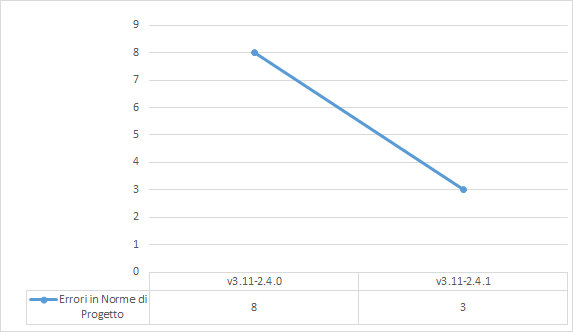
\includegraphics[width=10cm]{img/erroriNdPv3.11-2.4.1.png}
  \label{fig:errori_ndp}
  \caption{Grafico errori per \textsc{Norme di Progetto v3.11-2.4.1}}
\end{figure}

\begin{figure}[H]
  \centering
  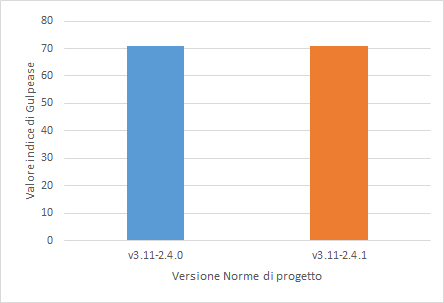
\includegraphics[width=10cm]{img/gulpeaseNdPv3.11-2.4.1.png}
  \label{fig:gulpease_ndp}
  \caption{Grafico indice di Gulpease per \textsc{Norme di Progetto v3.11-2.4.1}}
\end{figure}


\paragraph{Piano di Qualifica}
\label{sub:piano_di_qualifica}
Il \textsc{Piano di Qualifica v3.11-4.0.0} ha subito modifiche principalmente riguardanti i test e i valori delle metriche per la seguente fase.
Il suo indice di Gulpease si è assestato sul valore 72.

\rowcolors{2}{white!80!lightgray!90}{white}
\renewcommand{\arraystretch}{2} % allarga le righe con dello spazio sotto e sopra
\begin{longtable}[H]{>{\centering\bfseries}m{6cm} >{\centering}m{2cm} >{\centering}m{2.5cm} >{\centering}m{2.5cm} >{\centering\arraybackslash}m{2.5cm}}  
  \rowcolor{lightgray}
  {\textbf{Documento}} & {\textbf{Risultato indice}} & {\textbf{Errori presenti}} & {\textbf{Esito indice}} & {\textbf{Esito errori}}  \\
  \endfirsthead%
  \rowcolor{lightgray}
  {\textbf{Documento}} & {\textbf{Risultato indice}} & {\textbf{Errori presenti}} & {\textbf{Esito indice}} & {\textbf{Esito errori}}  \\
  \endhead%
  \textbf{Piano di Qualifica v3.11-4.0.0} & 72              & 0               & Soddisfatto & Soddisfatto \\
  \caption{Risultati metriche per il Piano di Qualifica v3.11-4.0.0}
  \label{tab:my-table}
\end{longtable}

\begin{figure}[H]
  \centering
  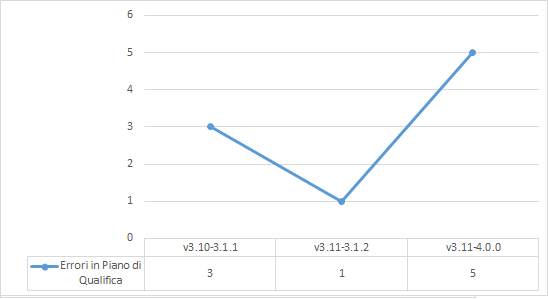
\includegraphics[width=10cm]{img/erroriPdQv3.11-4.0.0.png}
  \label{fig:errori_pdq}
  \caption{Grafico errori per \textsc{Piano di Qualifica v3.11-4.0.0}}
\end{figure}

\begin{figure}[H]
  \centering
  \includegraphics[width=10cm]{img/GulpeasePdQv3.11-4.0.0.png}
  \label{fig:gulpease_pdq}
  \caption{Grafico indice di Gulpease per \textsc{Piano di Qualifica v3.11-4.0.0}}
\end{figure}


\paragraph{Piano di Progetto}
\label{sub:piano_di_progetto}
Il \textsc{Piano di Progetto v1.9-4.2.0} ha subito parecchie modifiche che hanno richiesto molte fasi di verifica e approvazione che hanno sanato tutti gli errori.
Il suo indice di Gulpease è aumentato di 1 rispetto alla fase di sviluppo precedente.

\rowcolors{2}{white!80!lightgray!90}{white}
\renewcommand{\arraystretch}{2} % allarga le righe con dello spazio sotto e sopra
\begin{longtable}[H]{>{\centering\bfseries}m{6cm} >{\centering}m{2cm} >{\centering}m{2.5cm} >{\centering}m{2.5cm} >{\centering\arraybackslash}m{2.5cm}}  
  \rowcolor{lightgray}
  {\textbf{Documento}} & {\textbf{Risultato indice}} & {\textbf{Errori presenti}} & {\textbf{Esito indice}} & {\textbf{Esito errori}}  \\
  \endfirsthead%
  \rowcolor{lightgray}
  {\textbf{Documento}} & {\textbf{Risultato indice}} & {\textbf{Errori presenti}} & {\textbf{Esito indice}} & {\textbf{Esito errori}}  \\
  \endhead%
  \textbf{Piano di Progetto v1.9-4.2.0} & 73               & 0               & Soddisfatto & Soddisfatto \\
  \caption{Risultati metriche per il Piano di Progetto v1.9-4.2.0}
  \label{tab:my-table}
\end{longtable}

\begin{figure}[H]
  \centering
  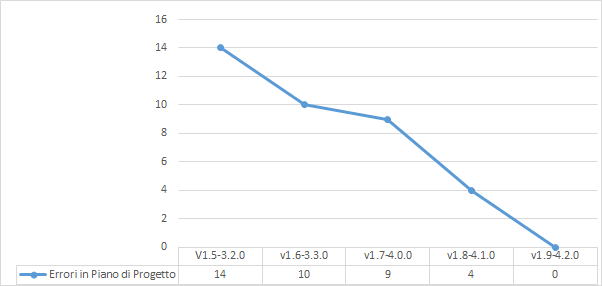
\includegraphics[width=10cm]{img/erroriPdPv1.9-4.2.0.png}
  \label{fig:errori_pdq}
  \caption{Grafico errori per \textsc{Piano di Progetto v1.9-4.2.0}}
\end{figure}

\begin{figure}[H]
  \centering
  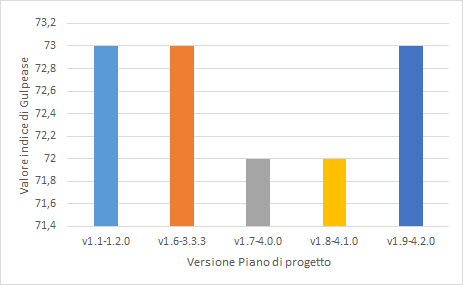
\includegraphics[width=10cm]{img/gulpeasePdPv1.9-4.2.0.png}
  \label{fig:gulpease_pdq}
  \caption{Grafico indice di Gulpease per \textsc{Piano di Progetto v1.9-4.2.0}}
\end{figure}


\paragraph{Analisi dei Requisiti}
\label{sub:analisi_dei_requisiti}
Le principali modifiche all'\textsc{Analisi dei Requisiti v1.9-1.3.0} riguardano l'aggiunta di nuovi casi d'uso e la modifica alla numerazione di certi requisiti, sono quindi state svolte solo 2 verifiche e approvazioni del documento.
Il suo indice di Gulpease è rimasto invariato rispetto alla fase di sviluppo precedente.

\rowcolors{2}{white!80!lightgray!90}{white}
\renewcommand{\arraystretch}{2} % allarga le righe con dello spazio sotto e sopra
\begin{longtable}[H]{>{\centering\bfseries}m{6cm} >{\centering}m{2cm} >{\centering}m{2.5cm} >{\centering}m{2.5cm} >{\centering\arraybackslash}m{2.5cm}}  
  \rowcolor{lightgray}
  {\textbf{Documento}} & {\textbf{Risultato indice}} & {\textbf{Errori presenti}} & {\textbf{Esito indice}} & {\textbf{Esito errori}}  \\
  \endfirsthead%
  \rowcolor{lightgray}
  {\textbf{Documento}} & {\textbf{Risultato indice}} & {\textbf{Errori presenti}} & {\textbf{Esito indice}} & {\textbf{Esito errori}}  \\
  \endhead%
  \textbf{Analisi dei Requisiti v1.9-1.3.0} &  73              & 0               & Soddisfatto & Soddisfatto \\
  \caption{Risultati metriche per l'Analisi dei Requisiti v1.9-1.3.0}
  \label{tab:my-table}
\end{longtable}

\begin{figure}[H]
  \centering
  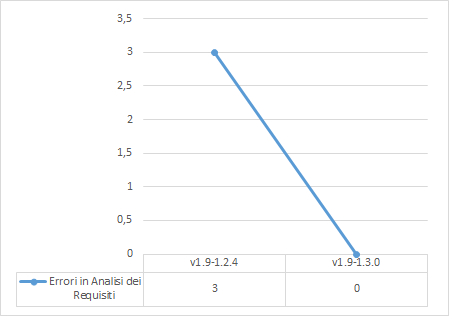
\includegraphics[width=10cm]{img/erroriAdRv1.9-1.3.0.png}
  \label{fig:errori_adr}
  \caption{Grafico errori per \textsc{Analisi dei Requisiti v1.9-1.3.0}}
\end{figure}

\begin{figure}[H]
  \centering
  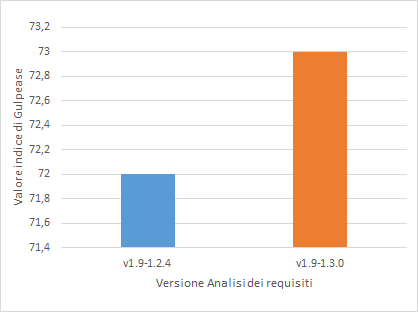
\includegraphics[width=10cm]{img/gulpeaseAdrv1.9-1.3.0.png}
  \label{fig:gulpease_adr}
  \caption{Grafico indice di Gulpease per \textsc{Analisi dei Requisiti v1.9-1.3.0}}
\end{figure}


\paragraph{Glossario}
\label{sub:glossario}
Il \textsc{Glossario v1.9-1.3.0} ha subito modifiche poco rilevanti per cui è bastata una sola revisione e approvazione generale al documento.
Il suo indice di Gulpease è rimasto invariato rispetto alla fase di sviluppo precedente.

\rowcolors{2}{white!80!lightgray!90}{white}
\renewcommand{\arraystretch}{2} % allarga le righe con dello spazio sotto e sopra
\begin{longtable}[H]{>{\centering\bfseries}m{6cm} >{\centering}m{2cm} >{\centering}m{2.5cm} >{\centering}m{2.5cm} >{\centering\arraybackslash}m{2.5cm}}  
  \rowcolor{lightgray}
  {\textbf{Documento}} & {\textbf{Risultato indice}} & {\textbf{Errori presenti}} & {\textbf{Esito indice}} & {\textbf{Esito errori}}  \\
  \endfirsthead%
  \rowcolor{lightgray}
  {\textbf{Documento}} & {\textbf{Risultato indice}} & {\textbf{Errori presenti}} & {\textbf{Esito indice}} & {\textbf{Esito errori}}  \\
  \endhead%
  \textbf{Glossario v1.9-1.3.0} & 65               & 0               & Soddisfatto & Soddisfatto \\
  \caption{Risultati metriche per il Glossario v1.9-1.3.0}
  \label{tab:my-table}
\end{longtable}

A causa delle poche modifiche e cambiamenti significativi non sono stati inseriti i grafici che non comunicavano alcuna informazione aggiuntiva.

\paragraph{Manuale Utente}
\label{sub:glossario}
Il \textsc{Manuale Utente v1.9-0.4.0} è stato redatto in questa fase di sviluppo e ha riportato moderati errori errori durante le sua verifiche che sono stati sanati.
Il suo indice di Gulpease in questa fase di sviluppo è 73.

\rowcolors{2}{white!80!lightgray!90}{white}
\renewcommand{\arraystretch}{2} % allarga le righe con dello spazio sotto e sopra
\begin{longtable}[H]{>{\centering\bfseries}m{6cm} >{\centering}m{2cm} >{\centering}m{2.5cm} >{\centering}m{2.5cm} >{\centering\arraybackslash}m{2.5cm}}  
  \rowcolor{lightgray}
  {\textbf{Documento}} & {\textbf{Risultato indice}} & {\textbf{Errori presenti}} & {\textbf{Esito indice}} & {\textbf{Esito errori}}  \\
  \endfirsthead%
  \rowcolor{lightgray}
  {\textbf{Documento}} & {\textbf{Risultato indice}} & {\textbf{Errori presenti}} & {\textbf{Esito indice}} & {\textbf{Esito errori}}  \\
  \endhead%
  \textbf{Manuale Utente v1.9-0.4.0} & 73               & 0               & Soddisfatto & Soddisfatto \\
  \caption{Risultati metriche per il Manuale Utente v1.9-0.4.0}
  \label{tab:my-table}
\end{longtable}

\begin{figure}[H]
  \centering
  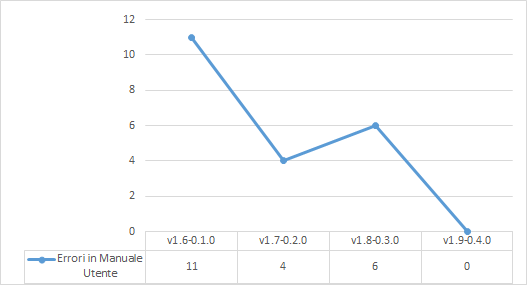
\includegraphics[width=10cm]{img/erroriMUv1.9-0.4.0.png}
  \label{fig:errori_adr}
  \caption{Grafico errori per \textsc{Manuale Utente v1.9-0.4.0}}
\end{figure}

\begin{figure}[H]
  \centering
  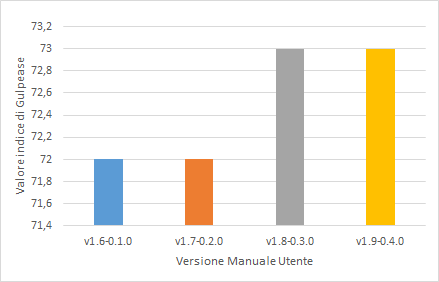
\includegraphics[width=10cm]{img/gulpeaseMUv1.9-0.4.0.png}
  \label{fig:gulpease_adr}
  \caption{Grafico indice di Gulpease per \textsc{Manuale Utente v1.9-0.4.0}}
\end{figure}

\paragraph{Manuale Sviluppatore}
\label{sub:glossario}
Il \textsc{Manuale Sviluppatore v1.9-1.0.0}, come per il \textsc{Manuale Utente v1.9-0.4.0}, è stato redatto in questa fase e ha avuto una curva di errori più altalenante che sono stati comunque sanati.
Il suo indice di Gulpease in questa fase di sviluppo è 71.

\rowcolors{2}{white!80!lightgray!90}{white}
\renewcommand{\arraystretch}{2} % allarga le righe con dello spazio sotto e sopra
\begin{longtable}[H]{>{\centering\bfseries}m{6cm} >{\centering}m{2cm} >{\centering}m{2.5cm} >{\centering}m{2.5cm} >{\centering\arraybackslash}m{2.5cm}}  
  \rowcolor{lightgray}
  {\textbf{Documento}} & {\textbf{Risultato indice}} & {\textbf{Errori presenti}} & {\textbf{Esito indice}} & {\textbf{Esito errori}}  \\
  \endfirsthead%
  \rowcolor{lightgray}
  {\textbf{Documento}} & {\textbf{Risultato indice}} & {\textbf{Errori presenti}} & {\textbf{Esito indice}} & {\textbf{Esito errori}}  \\
  \endhead%
  \textbf{Manuale Sviluppatore v1.9-1.0.0} & 71               & 0               & Soddisfatto & Soddisfatto \\
  \caption{Risultati metriche per il Manuale Sviluppatore v1.9-1.0.0}
  \label{tab:my-table}
\end{longtable}

\begin{figure}[H]
  \centering
  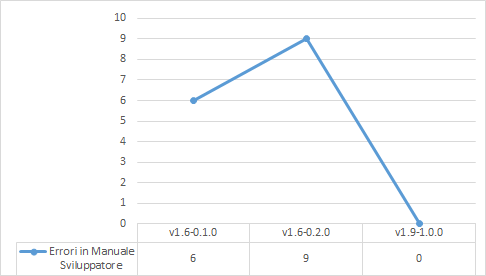
\includegraphics[width=10cm]{img/erroriMSv1.9-1.0.0.png}
  \label{fig:errori_adr}
  \caption{Grafico errori per \textsc{Manuale Sviluppatore v1.9-1.0.0}}
\end{figure}

\begin{figure}[H]
  \centering
  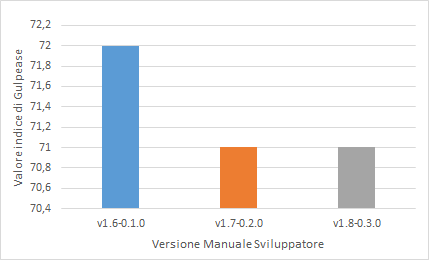
\includegraphics[width=10cm]{img/gulpeaseMSv1.9-1.0.0.png}
  \label{fig:gulpease_adr}
  \caption{Grafico indice di Gulpease per \textsc{Manuale Sviluppatore v1.9-1.0.0}}
\end{figure}

\subsubsection{Esiti verifiche sui processi}
\label{sub:esiti_verifiche_sui_processi}
In questa sezione vengono visualizzati gli esiti delle metriche prese in considerazione per quanto riguarda i processi produttivi.
Come per i documenti, anche per queste metriche verrà fornito un esito che può essere soddisfacente o meno.

\paragraph{Processo PRC001}
\label{sub:processo_PRC001}

\rowcolors{2}{white!80!lightgray!90}{white}
\renewcommand{\arraystretch}{2} % allarga le righe con dello spazio sotto e sopra
\begin{longtable}[H]{>{\centering\bfseries}m{5cm} >{\centering}m{5cm} >{\centering}m{2.5cm} >{\centering\arraybackslash}m{2.5cm}}  
  \rowcolor{lightgray}
  {\textbf{Obiettivo}} & {\textbf{Metrica}} & {\textbf{Risultato}} & {\textbf{Esito}}  \\
  \endfirsthead%
  \rowcolor{lightgray}
  {\textbf{Obiettivo}} & {\textbf{Metrica}} & {\textbf{Risultato}} & {\textbf{Esito}}  \\
  \endhead%
  \textbf{QoPR001 Rispetto delle scadenze della pianificazione} & MoPR001 Varianza dei tempi &  1.02 & Soddisfatto  \\
  \caption{Risultati metrica MoPR001}
  \label{tab:my-table}
\end{longtable}
\textbf{Nota}: I ritardi nelle scadenze pianificate sono diminuiti nel corso di quest'ultima fase di progetto.

\rowcolors{2}{white!80!lightgray!90}{white}
\renewcommand{\arraystretch}{2} % allarga le righe con dello spazio sotto e sopra
\begin{longtable}[H]{>{\centering\bfseries}m{5cm} >{\centering}m{5cm} >{\centering}m{2.5cm} >{\centering\arraybackslash}m{2.5cm}}  
  \rowcolor{lightgray}
  {\textbf{Obiettivo}} & {\textbf{Metrica}} & {\textbf{Risultato}} & {\textbf{Esito}}  \\
  \endfirsthead%
  \rowcolor{lightgray}
  {\textbf{Obiettivo}} & {\textbf{Metrica}} & {\textbf{Risultato}} & {\textbf{Esito}}  \\
  \endhead%
  \textbf{QoPR002 Rispetto del budget istanziato} & MoPR002 Varianza dei costi &  & Soddisfatto  \\
  \caption{Risultati metrica MoPR002}
  \label{tab:my-table}
\end{longtable}
\textbf{Nota}: La variazione rispetto al preventivo iniziale rientra nel range deciso per la metrica, per cui l'obiettivo è stato soddisfatto. Il discostamento dal preventivo totale rilevato è di:  euro.

\rowcolors{2}{white!80!lightgray!90}{white}
\renewcommand{\arraystretch}{2} % allarga le righe con dello spazio sotto e sopra
\begin{longtable}[H]{>{\centering\bfseries}m{5cm} >{\centering}m{5cm} >{\centering}m{2.5cm} >{\centering\arraybackslash}m{2.5cm}}  
  \rowcolor{lightgray}
  {\textbf{Obiettivo}} & {\textbf{Metrica}} & {\textbf{Risultato}} & {\textbf{Esito}}  \\
  \endfirsthead%
  \rowcolor{lightgray}
  {\textbf{Obiettivo}} & {\textbf{Metrica}} & {\textbf{Risultato}} & {\textbf{Esito}}  \\
  \endhead%
  \textbf{QoPR003 Rispetto del ciclo di vita scelto} & MoPR003 Aderenza agli standard & Livello di maturità: 3 \\ Valutazione attributi: L  &  Soddisfatto \\
  \caption{Risultati metrica MoPR003}
  \label{tab:my-table}
\end{longtable}
\textbf{Nota}: IL miglioramento per quanto riguarda l'aderenza agli standard è rimasto costante anche in questa fase.

\rowcolors{2}{white!80!lightgray!90}{white}
\renewcommand{\arraystretch}{2} % allarga le righe con dello spazio sotto e sopra
\begin{longtable}[H]{>{\centering\bfseries}m{5cm} >{\centering}m{5cm} >{\centering}m{2.5cm} >{\centering\arraybackslash}m{2.5cm}}  
  \rowcolor{lightgray}
  {\textbf{Obiettivo}} & {\textbf{Metrica}} & {\textbf{Risultato}} & {\textbf{Esito}}  \\
  \endfirsthead%
  \rowcolor{lightgray}
  {\textbf{Obiettivo}} & {\textbf{Metrica}} & {\textbf{Risultato}} & {\textbf{Esito}}  \\
  \endhead%
  \textbf{QoPR004 Rispetto dei ruoli e identificazione nei prodotti} & MoPR004 Aderenza ai ruoli & 0 & Soddisfatto \\
  \caption{Risultati metrica MoPR004}
  \label{tab:my-table}
\end{longtable}
\textbf{Nota}: In ogni documento prodotto i ruoli sono stati identificati e rispettati.

\rowcolors{2}{white!80!lightgray!90}{white}
\renewcommand{\arraystretch}{2} % allarga le righe con dello spazio sotto e sopra
\begin{longtable}[H]{>{\centering\bfseries}m{5cm} >{\centering}m{5cm} >{\centering}m{2.5cm} >{\centering\arraybackslash}m{2.5cm}}  
  \rowcolor{lightgray}
  {\textbf{Obiettivo}} & {\textbf{Metrica}} & {\textbf{Risultato}} & {\textbf{Esito}}  \\
  \endfirsthead%
  \rowcolor{lightgray}
  {\textbf{Obiettivo}} & {\textbf{Metrica}} & {\textbf{Risultato}} & {\textbf{Esito}}  \\
  \endhead%
  \textbf{QoPR005 Rispetto del versionamento dei prodotti} & MoPR005 Controllo prodotti & 25.8 & Soddisfatto \\
  \caption{Risultati metrica MoPR005}
  \label{tab:my-table}
\end{longtable}
\textbf{Nota}: Il numero di commit in questa fase è stato parecchio elevato, il che soddisfa appieno l'obiettivo prefissato.

\paragraph{Processo PRC002}
\label{sub:processo_PRC002}

\rowcolors{2}{white!80!lightgray!90}{white}
\renewcommand{\arraystretch}{2} % allarga le righe con dello spazio sotto e sopra
\begin{longtable}[H]{>{\centering\bfseries}m{5cm} >{\centering}m{5cm} >{\centering}m{2.5cm} >{\centering\arraybackslash}m{2.5cm}}  
  \rowcolor{lightgray}
  {\textbf{Obiettivo}} & {\textbf{Metrica}} & {\textbf{Risultato}} & {\textbf{Esito}}  \\
  \endfirsthead%
  \rowcolor{lightgray}
  {\textbf{Obiettivo}} & {\textbf{Metrica}} & {\textbf{Risultato}} & {\textbf{Esito}}  \\
  \endhead%
  \textbf{QoPR006 Soddisfazione dei requisiti obbligatori} & MoPR006 Verifica requisiti obbligatori & 100\% & Non soddisfatto \\
  \caption{Risultati metrica MoPR006}
  \label{tab:my-table}
\end{longtable}
\textbf{Nota}: Tutti i requisiti obbligatori sono stati soddisfatti per questa revisione finale.

\rowcolors{2}{white!80!lightgray!90}{white}
\renewcommand{\arraystretch}{2} % allarga le righe con dello spazio sotto e sopra
\begin{longtable}[H]{>{\centering\bfseries}m{5cm} >{\centering}m{5cm} >{\centering}m{2.5cm} >{\centering\arraybackslash}m{2.5cm}}  
  \rowcolor{lightgray}
  {\textbf{Obiettivo}} & {\textbf{Metrica}} & {\textbf{Risultato}} & {\textbf{Esito}}  \\
  \endfirsthead%
  \rowcolor{lightgray}
  {\textbf{Obiettivo}} & {\textbf{Metrica}} & {\textbf{Risultato}} & {\textbf{Esito}}  \\
  \endhead%
  \textbf{QoPR007 Soddisfazione dei requisiti opzionali e desiderabili} & MoPR007 Verifica requisiti opzionali \\ MoPR008 Verifica requisiti desiderabili &  & Non soddisfatto \\
  \caption{Risultati metrica MoPR007 e metrica MoPR008}
  \label{tab:my-table}
\end{longtable}
\textbf{Nota}: 

\rowcolors{2}{white!80!lightgray!90}{white}
\renewcommand{\arraystretch}{2} % allarga le righe con dello spazio sotto e sopra
\begin{longtable}[H]{>{\centering\bfseries}m{5cm} >{\centering}m{5cm} >{\centering}m{2.5cm} >{\centering\arraybackslash}m{2.5cm}}  
  \rowcolor{lightgray}
  {\textbf{Obiettivo}} & {\textbf{Metrica}} & {\textbf{Risultato}} & {\textbf{Esito}}  \\
  \endfirsthead%
  \rowcolor{lightgray}
  {\textbf{Obiettivo}} & {\textbf{Metrica}} & {\textbf{Risultato}} & {\textbf{Esito}}  \\
  \endhead%
  \textbf{QoPR008 Verifica dei rischi previsti} & MoPR009 Verifica rischi non pervenuti & 0 & Soddisfatto \\
  \caption{Risultati metrica MoPR009}
  \label{tab:my-table}
\end{longtable}
\textbf{Nota}: Non sono ancora stati rivelati rischi importanti che non siano stati previsti precedentemente dal gruppo.

\paragraph{Processo PRC003}
\label{sub:processo_PRC003}

\rowcolors{2}{white!80!lightgray!90}{white}
\renewcommand{\arraystretch}{2} % allarga le righe con dello spazio sotto e sopra
\begin{longtable}[H]{>{\centering\bfseries}m{5cm} >{\centering}m{5cm} >{\centering}m{2.5cm} >{\centering\arraybackslash}m{2.5cm}}  
  \rowcolor{lightgray}
  {\textbf{Obiettivo}} & {\textbf{Metrica}} & {\textbf{Risultato}} & {\textbf{Esito}}  \\
  \endfirsthead%
  \rowcolor{lightgray}
  {\textbf{Obiettivo}} & {\textbf{Metrica}} & {\textbf{Risultato}} & {\textbf{Esito}}  \\
  \endhead%
  \textbf{QoPR09 Rispetto delle fasi del ciclo di vita} & MoPR010 Analisi Way of Working & / & Soddisfatto \\
  \caption{Risultati metrica MoPR010}
  \label{tab:my-table}
\end{longtable}
\textbf{Nota}: I componenti del gruppo svolgono costantemente un aggiornamento in base alle modifiche fatte alle \textsc{Norme di Progetto}.

\rowcolors{2}{white!80!lightgray!90}{white}
\renewcommand{\arraystretch}{2} % allarga le righe con dello spazio sotto e sopra
\begin{longtable}[H]{>{\centering\bfseries}m{5cm} >{\centering}m{5cm} >{\centering}m{2.5cm} >{\centering\arraybackslash}m{2.5cm}}  
  \rowcolor{lightgray}
  {\textbf{Obiettivo}} & {\textbf{Metrica}} & {\textbf{Risultato}} & {\textbf{Esito}}  \\
  \endfirsthead%
  \rowcolor{lightgray}
  {\textbf{Obiettivo}} & {\textbf{Metrica}} & {\textbf{Risultato}} & {\textbf{Esito}}  \\
  \endhead%
  \textbf{QoPR010 Rispetto nella redazione dei documenti} & MoPR011 Analisi documenti & 3 & Soddisfatto \\
  \caption{Risultati metrica MoPR011}
  \label{tab:my-table}
\end{longtable}
\textbf{Nota}: Anche se nei documenti sono state apportate poche modifiche mediamente ogni documento è stato revisionato e approvato 3 volte.

\paragraph{Processo PRC004}
\label{sub:processo_PRC004}

\rowcolors{2}{white!80!lightgray!90}{white}
\renewcommand{\arraystretch}{2} % allarga le righe con dello spazio sotto e sopra
\begin{longtable}[H]{>{\centering\bfseries}m{5cm} >{\centering}m{5cm} >{\centering}m{2.5cm} >{\centering\arraybackslash}m{2.5cm}}  
  \rowcolor{lightgray}
  {\textbf{Obiettivo}} & {\textbf{Metrica}} & {\textbf{Risultato}} & {\textbf{Esito}}  \\
  \endfirsthead%
  \rowcolor{lightgray}
  {\textbf{Obiettivo}} & {\textbf{Metrica}} & {\textbf{Risultato}} & {\textbf{Esito}}  \\
  \endhead%
  \textbf{QoPR011 Attuare una verifica costante} & MoPR012 Frequenza di controlli & / & Soddisfatto \\
  \caption{Risultati metrica MoPR012}
  \label{tab:my-table}
\end{longtable}
\textbf{Nota}: I verificatori stanno continuando ad effettuare delle verifiche costanti ai prodotti.


\rowcolors{2}{white!80!lightgray!90}{white}
\renewcommand{\arraystretch}{2} % allarga le righe con dello spazio sotto e sopra
\begin{longtable}[H]{>{\centering\bfseries}m{5cm} >{\centering}m{5cm} >{\centering}m{2.5cm} >{\centering\arraybackslash}m{2.5cm}}  
  \rowcolor{lightgray}
  {\textbf{Obiettivo}} & {\textbf{Metrica}} & {\textbf{Risultato}} & {\textbf{Esito}}  \\
  \endfirsthead%
  \rowcolor{lightgray}
  {\textbf{Obiettivo}} & {\textbf{Metrica}} & {\textbf{Risultato}} & {\textbf{Esito}}  \\
  \endhead%
  \textbf{QoPR013 Rispettare le fasi di verifica} & MoPR010 Analisi Way of Working & / & Soddisfatto \\
  \caption{Risultati QoPR13}
  \label{tab:my-table}
\end{longtable}
\textbf{Nota}: Le fasi di verifica dei prodotti stanno vedendo rispettate secondo le indicazioni interne al gruppo.

\rowcolors{2}{white!80!lightgray!90}{white}
\renewcommand{\arraystretch}{2} % allarga le righe con dello spazio sotto e sopra
\begin{longtable}[H]{>{\centering\bfseries}m{5cm} >{\centering}m{5cm} >{\centering}m{2.5cm} >{\centering\arraybackslash}m{2.5cm}}  
  \rowcolor{lightgray}
  {\textbf{Obiettivo}} & {\textbf{Metrica}} & {\textbf{Risultato}} & {\textbf{Esito}}  \\
  \endfirsthead%
  \rowcolor{lightgray}
  {\textbf{Obiettivo}} & {\textbf{Metrica}} & {\textbf{Risultato}} & {\textbf{Esito}}  \\
  \endhead%
  \textbf{QoPR014 Soddisfare i test richiesti} & MoPR013 Percentuale di test soddisfatti & 85\% & Non soddisfatto \\
  \caption{Risultati MoPR013}
  \label{tab:my-table}
\end{longtable}
\textbf{Nota}:  Come preventivato, in questa ultima fase di progetto siamo riusciti ad ottenere un valore accettabile per quanto riguarda il numero di test implementati.

\begin{figure}[H]
  \centering
  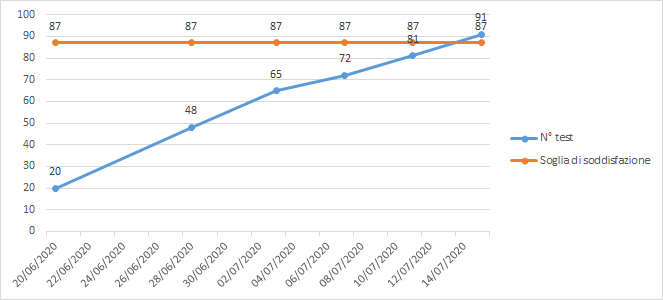
\includegraphics[width=12cm]{img/testImplRa.png}
  \label{fig:test_implementati}
  \caption{Grafico con il numero test implementati}
\end{figure}

\subsubsection{Esiti verifiche sui prodotti}

\label{sub:esiti_verifiche_sui_prodotti}
In questa sezione vengono visualizzati gli esiti delle metriche prese in considerazione per quanto riguarda i prodotti realizzati. Come per i documenti, anche per queste metriche verrà fornito un esito che può essere soddisfacente o meno.

\paragraph{Funzionalità}
\label{sub:funzionalita}

\rowcolors{2}{white!80!lightgray!90}{white}
\renewcommand{\arraystretch}{2} % allarga le righe con dello spazio sotto e sopra
\begin{longtable}[H]{>{\centering\bfseries}m{5cm} >{\centering}m{5cm} >{\centering}m{2.5cm} >{\centering\arraybackslash}m{2.5cm}}  
  \rowcolor{lightgray}
  {\textbf{Obiettivo}} & {\textbf{Metrica}} & {\textbf{Risultato}} & {\textbf{Esito}}  \\
  \endfirsthead%
  \rowcolor{lightgray}
  {\textbf{Obiettivo}} & {\textbf{Metrica}} & {\textbf{Risultato}} & {\textbf{Esito}}  \\
  \endhead%
  \textbf{QoPD001 Rispetto dell’implementazione funzionale - [Adeguatezza]} & MoPD001 Completezza di implementazione - [Adeguatezza] & 0 & Soddisfatto \\
  \caption{Risultati metrica MoPD001}
  \label{tab:my-table}
\end{longtable}
\textbf{Nota}: Tutte le funzioni da implementare in questa fase sono state implementate.

\rowcolors{2}{white!80!lightgray!90}{white}
\renewcommand{\arraystretch}{2} % allarga le righe con dello spazio sotto e sopra
\begin{longtable}[H]{>{\centering\bfseries}m{5cm} >{\centering}m{5cm} >{\centering}m{2.5cm} >{\centering\arraybackslash}m{2.5cm}}  
  \rowcolor{lightgray}
  {\textbf{Obiettivo}} & {\textbf{Metrica}} & {\textbf{Risultato}} & {\textbf{Esito}}  \\
  \endfirsthead%
  \rowcolor{lightgray}
  {\textbf{Obiettivo}} & {\textbf{Metrica}} & {\textbf{Risultato}} & {\textbf{Esito}}  \\
  \endhead%
  \textbf{QoPD002 Rispetto delle interfacce - [Interoperabilità]} & MoPD002 Coerenza di interfaccia - [Interoperabilità] & 92\% & Soddisfatto \\
  \caption{Risultati metrica MoPD002}
  \label{tab:my-table}
\end{longtable}
\textbf{Nota}: il 92\% delle interfacce realizzate è fedele a quanto preventivamente definito.

\paragraph{Affidabilità}
\label{sub:affidabilita}

\rowcolors{2}{white!80!lightgray!90}{white}
\renewcommand{\arraystretch}{2} % allarga le righe con dello spazio sotto e sopra
\begin{longtable}[H]{>{\centering\bfseries}m{5cm} >{\centering}m{5cm} >{\centering}m{2.5cm} >{\centering\arraybackslash}m{2.5cm}}  
  \rowcolor{lightgray}
  {\textbf{Obiettivo}} & {\textbf{Metrica}} & {\textbf{Risultato}} & {\textbf{Esito}}  \\
  \endfirsthead%
  \rowcolor{lightgray}
  {\textbf{Obiettivo}} & {\textbf{Metrica}} & {\textbf{Risultato}} & {\textbf{Esito}}  \\
  \endhead%
  \textbf{QoPD003 Test completi sul codice - [Maturità]} & MoPD003 Copertura dei test- [Maturità] &  & Non soddisfatto \\
  \caption{Risultati metrica MoPD003}
  \label{tab:my-table}
\end{longtable}
\textbf{Nota}: 

\rowcolors{2}{white!80!lightgray!90}{white}
\renewcommand{\arraystretch}{2} % allarga le righe con dello spazio sotto e sopra
\begin{longtable}[H]{>{\centering\bfseries}m{5cm} >{\centering}m{5cm} >{\centering}m{2.5cm} >{\centering\arraybackslash}m{2.5cm}}  
  \rowcolor{lightgray}
  {\textbf{Obiettivo}} & {\textbf{Metrica}} & {\textbf{Risultato}} & {\textbf{Esito}}  \\
  \endfirsthead%
  \rowcolor{lightgray}
  {\textbf{Obiettivo}} & {\textbf{Metrica}} & {\textbf{Risultato}} & {\textbf{Esito}}  \\
  \endhead%
  \textbf{QoPD004 Individuazione test falliti - [Affidabilità]} & MoPD004 Densità degli errori - [Affidabilità] & 5\% & Soddisfatto \\
  \caption{Risultati metrica MoPD004}
  \label{tab:my-table}
\end{longtable}
\textbf{Nota}: Al momento il numero dei test ha prodotto errori solo nel 5\% dei casi il che è un valore accettabile dal gruppo.

\paragraph{Usabilità}
\label{sub:usabilita}

\rowcolors{2}{white!80!lightgray!90}{white}
\renewcommand{\arraystretch}{2} % allarga le righe con dello spazio sotto e sopra
\begin{longtable}[H]{>{\centering\bfseries}m{5cm} >{\centering}m{5cm} >{\centering}m{2.5cm} >{\centering\arraybackslash}m{2.5cm}}  
  \rowcolor{lightgray}
  {\textbf{Obiettivo}} & {\textbf{Metrica}} & {\textbf{Risultato}} & {\textbf{Esito}}  \\
  \endfirsthead%
  \rowcolor{lightgray}
  {\textbf{Obiettivo}} & {\textbf{Metrica}} & {\textbf{Risultato}} & {\textbf{Esito}}  \\
  \endhead%
  \textbf{QoPD005 Chiarezza del comportamento - [Comprensibilità]} & MoPD005 Documentazione delle funzioni - [Comprensibilità] & 90\%  & Soddisfatto \\
  \caption{Risultati metrica MoPD005}
  \label{tab:my-table}
\end{longtable}
\textbf{Nota}: Quasi tutte le funzioni implementate sono state descritte con un commento, tranne le funzioni che non richiedono particolare spiegazione.

\rowcolors{2}{white!80!lightgray!90}{white}
\renewcommand{\arraystretch}{2} % allarga le righe con dello spazio sotto e sopra
\begin{longtable}[H]{>{\centering\bfseries}m{5cm} >{\centering}m{5cm} >{\centering}m{2.5cm} >{\centering\arraybackslash}m{2.5cm}}  
  \rowcolor{lightgray}
  {\textbf{Obiettivo}} & {\textbf{Metrica}} & {\textbf{Risultato}} & {\textbf{Esito}}  \\
  \endfirsthead%
  \rowcolor{lightgray}
  {\textbf{Obiettivo}} & {\textbf{Metrica}} & {\textbf{Risultato}} & {\textbf{Esito}}  \\
  \endhead%
  \textbf{QoPD006 Chiarimento degli errori - [Comprensibilità]} & MoPD006 Messaggi di errore - [Comprensibilità] & 6\% & Soddisfatto \\
  \caption{Risultati metrica MoPD006}
  \label{tab:my-table}
\end{longtable}
\textbf{Nota}: Il valore è migliorate in quest'ultima fase e rimane soddisfacente per il gruppo.

\paragraph{Efficienza}
\label{sub:efficienza}

\rowcolors{2}{white!80!lightgray!90}{white}
\renewcommand{\arraystretch}{2} % allarga le righe con dello spazio sotto e sopra
\begin{longtable}[H]{>{\centering\bfseries}m{5cm} >{\centering}m{5cm} >{\centering}m{2.5cm} >{\centering\arraybackslash}m{2.5cm}}  
  \rowcolor{lightgray}
  {\textbf{Obiettivo}} & {\textbf{Metrica}} & {\textbf{Risultato}} & {\textbf{Esito}}  \\
  \endfirsthead%
  \rowcolor{lightgray}
  {\textbf{Obiettivo}} & {\textbf{Metrica}} & {\textbf{Risultato}} & {\textbf{Esito}}  \\
  \endhead%
  \textbf{QoPD007 Velocità di esecuzione - [Comportamento temporale]} & MoPD007 Tempo medio di risposta - [Comportamento temporale] & 1.66 & Soddisfatto \\
  \caption{Risultati metrica MoPD007}
  \label{tab:my-table}
\end{longtable}
\textbf{Nota}: Il tempo di risposta soddisfa le aspettative di qualità per la metrica per essendo leggermente aumentato.
\paragraph{Manutenibilità}
\label{sub:manutenibilita}

\rowcolors{2}{white!80!lightgray!90}{white}
\renewcommand{\arraystretch}{2} % allarga le righe con dello spazio sotto e sopra
\begin{longtable}[H]{>{\centering\bfseries}m{5cm} >{\centering}m{5cm} >{\centering}m{2.5cm} >{\centering\arraybackslash}m{2.5cm}}  
  \rowcolor{lightgray}
  {\textbf{Obiettivo}} & {\textbf{Metrica}} & {\textbf{Risultato}} & {\textbf{Esito}}  \\
  \endfirsthead%
  \rowcolor{lightgray}
  {\textbf{Obiettivo}} & {\textbf{Metrica}} & {\textbf{Risultato}} & {\textbf{Esito}}  \\
  \endhead%
  \textbf{QoPD08 Comprensione del codice - [Modifica]} & MoPD008 Commenti sul codice - [Modifica] &  & Soddisfatto \\
  \caption{Risultati metrica MoPD006}
  \label{tab:my-table}
\end{longtable}
\textbf{Nota}:

\subsubsection{Conclusioni}%
\label{sub:conclusioni}
In questa fase il team ha provveduto principalmente a sanare le lacune riguardanti l'implementazione dei test che risultavano essere carenti nella fase di sviluppo precedente.
